\section{Introduction}

\begin{frame}
	\frametitle{What's RoboCup}
	
	\vspace{0.5cm}
	
	\begin{block}{RoboCup}
		``RoboCup is an international scientific initiative with the goal to advance the
		state-of-the-art of intelligent robots. When established in 1997, the original mission
		was to field a team of robots capable of winning against the human soccer World Cup
		Champions by 2050.''
	\end{block}
	
	\vspace{0.05cm}
	
	\begin{figure}[!t]
		\centering
		\begin{tikzpicture}[map/.style={draw=black,ultra thick,inner sep=0pt}]
			\node at (0,0) [map]
			{
				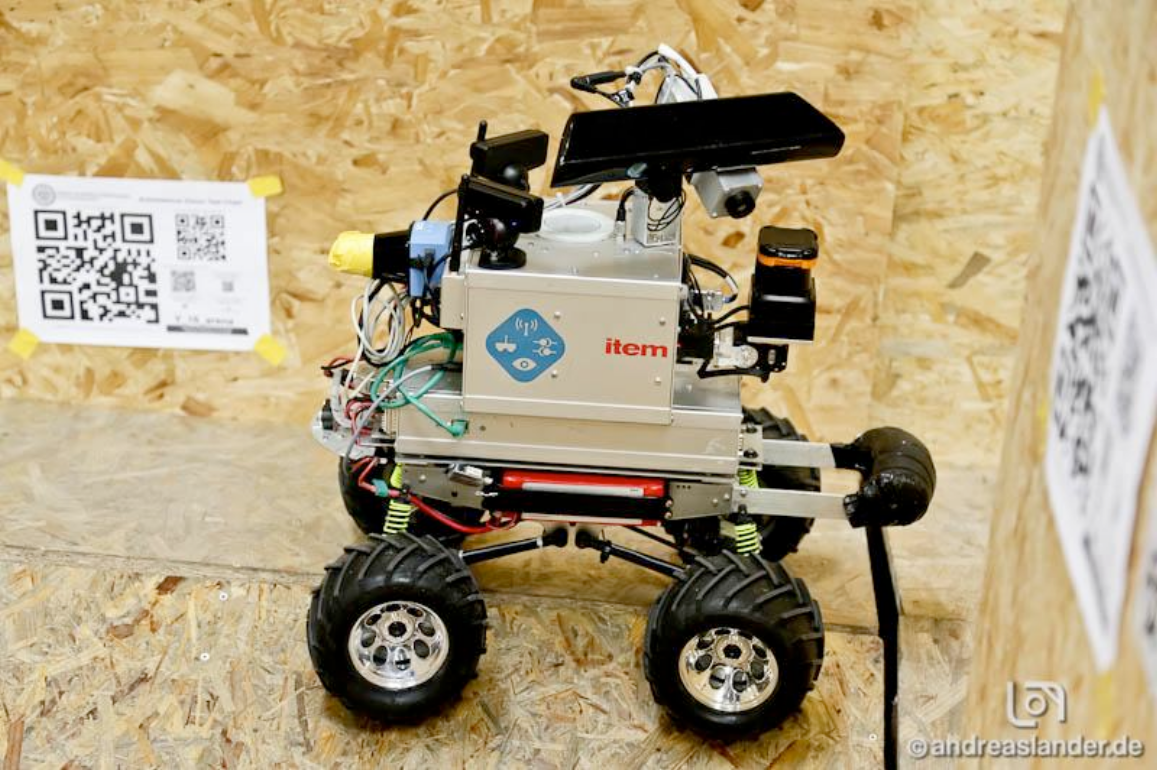
\includegraphics[height=3cm]{Figures/RoboCup-1}
			};
			\node at (3.62,0) [map]
			{
				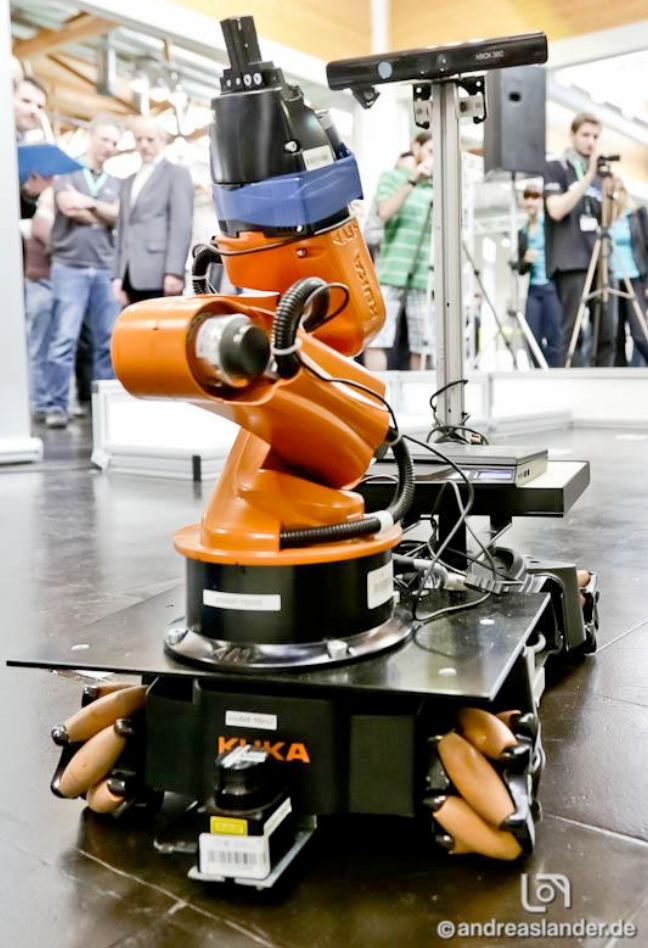
\includegraphics[height=3cm]{Figures/RoboCup-2}
			};
			\node at (7,0) [map]
			{
				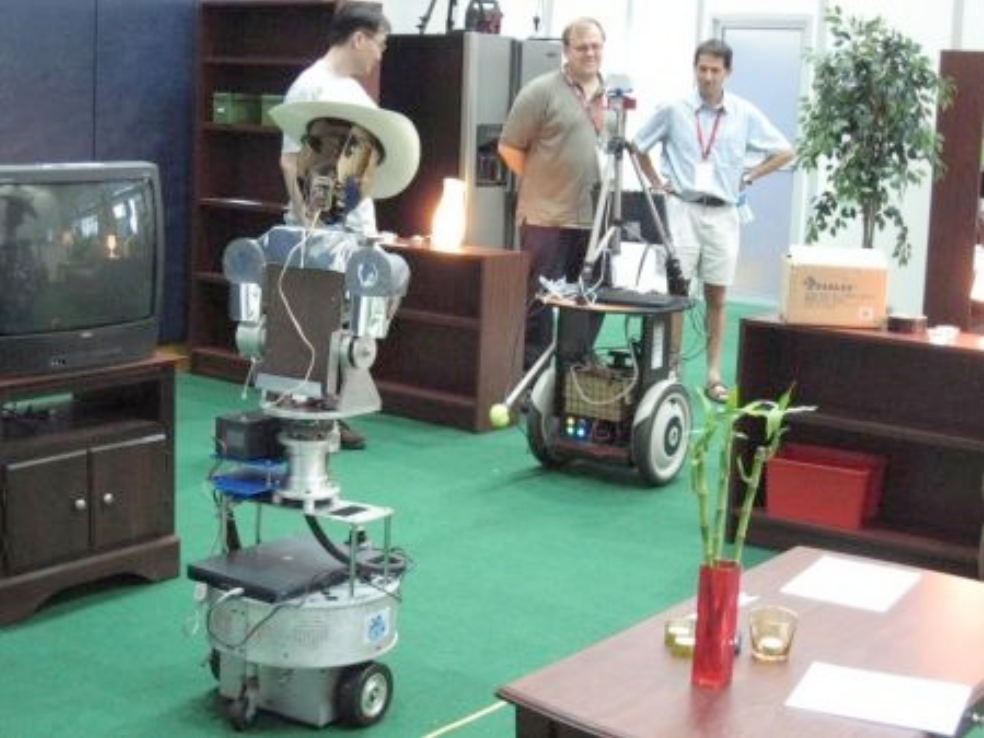
\includegraphics[height=3cm]{Figures/RoboCup-3}
			};
		\end{tikzpicture}
	\end{figure}
	
	\vspace{-0.4cm}
	
	\begin{tabbing}
		\hspace{2cm}
		Rescue
		\hspace{2.15cm}
		\MVAt Work
		\hspace{1.85cm}
		\MVAt Home
	\end{tabbing}
\end{frame}

\begin{frame}
	\frametitle{Challenge}
	
	\Large
	
	\vspace{0.25cm}
	
	\begin{figure}
		\centering
		\begin{tikzpicture}
			\node at (0,0) [draw=white,ultra thick,inner sep=0pt]
			{
				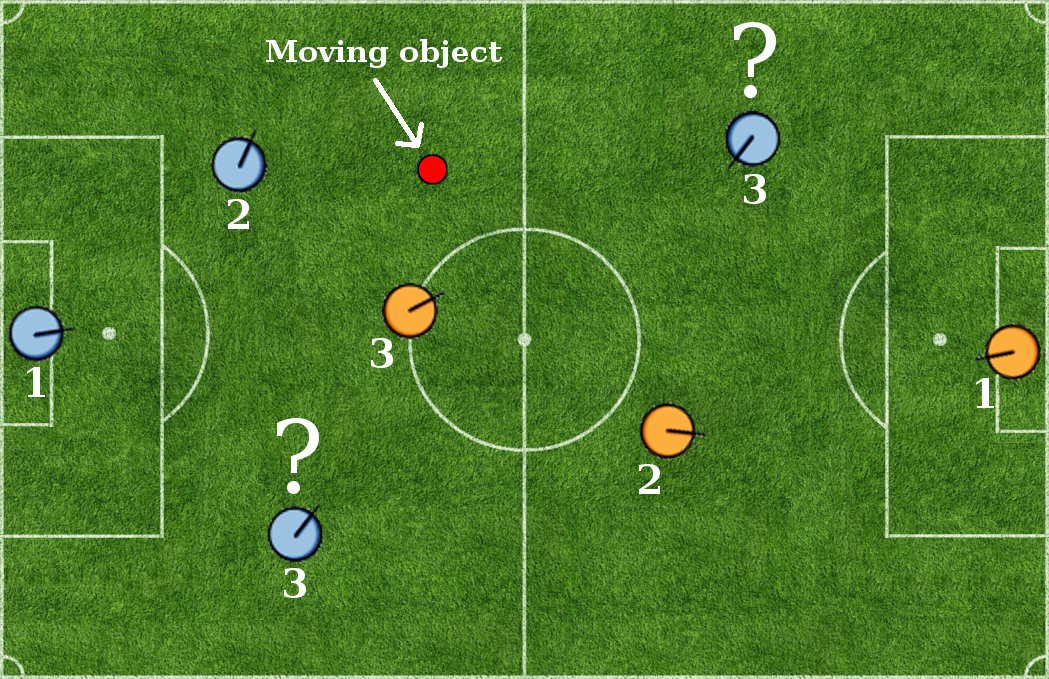
\includegraphics[width=0.8\linewidth]{Figures/Challenge}
			};
		\end{tikzpicture}
	\end{figure}
	
	\vspace{-0.4cm}
	
	\begin{center}
		What is the real position of the blue robot number 3?
	\end{center}
\end{frame}

\begin{frame}
	\frametitle{Motivation}
	
	\Large
	
	\vspace{0.2cm}
	
	Considerable contribution to the development of an effective play for the next winning
	teams.
	
	\vspace{-0.2cm}
	
	\begin{figure}[!t]
		\centering
		\begin{tikzpicture}[map/.style={draw=black,ultra thick,inner sep=0pt}]
			\node at (0,0) [map]
			{
				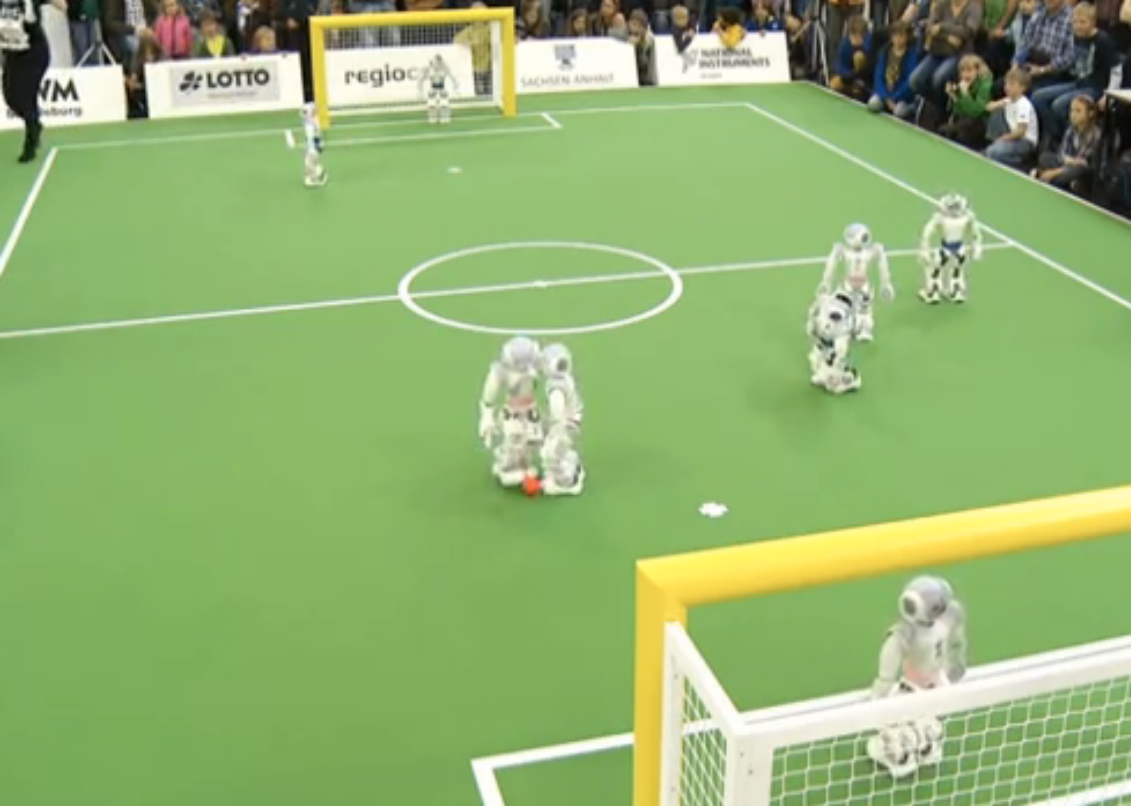
\includegraphics[height=4cm]{Figures/Flipped}
			};
		\end{tikzpicture}
	\end{figure}
	
	\vspace{-0.37cm}
	
	Develop a disambiguation technique, robust to noise and false perceptions, exploiting  the
	\textbf{PTracking} algorithm.\\
\end{frame}

\begin{frame}
	\frametitle{Related Work}
	
	\vspace{0.4cm}
	
	\large
	
	Two major different approaches have been presented so far:
	
	\begin{itemize}
		\item \textbf{Background noise analysis:} the rUNSWift SPL team exploited the background 
			  noise of two images taken at the beginning of the game [Harris and Anderson, 2012]
		\vspace{0.15cm}
		\item \textbf{Robot information sharing:} comparison between the different models of
			  the ball position and the robots' world beliefs. In particular:
			  
			  \begin{itemize}
			  	  \item the Austin-Villa team used a counter to keep track of the different ball
			  	  		estimations [Barret and Genter, 2013]
			  	  \vspace{0.1cm}
			  	  \item the B-Human team exploited a fused ball model to check every robot field
						representation [R\"{o}fer and Laue, 2012]
			  \end{itemize}
	\end{itemize}
\end{frame}
